\documentclass[11pt]{article} % use larger type; default would be 10pt

\usepackage[utf8]{inputenc} % set input encoding (not needed with XeLaTeX)

\usepackage{tikz}
\begin{document}
\tikz[%every node/.style={black},
	   dot/.style={font=\tiny},
	  every circle/.style={fill,black}] {
\path[use as bounding box, red] (-3,0) rectangle (2,1);
\path[fill,blue!20] 
	(0,0) -- (1, 0) -- (2, 0) 
	-- (2, 1) --  (2, 2) -- (1, 2) -- (0, 2); 
\fill (0,2) circle(1.5pt)
	node[anchor=south east]{north west};
\fill (1, 2) circle(1.5pt)
	node[anchor=south]{north};
\fill (2, 2) circle(1.5pt)
	node[anchor=south west] {north east};
\fill (2, 1) circle(1.5pt)
	node[anchor=west] {east};
\fill (2, 0) circle(1.5pt)
	node[anchor=north west] {south east};
\fill (1, 0) circle(1.5pt)
	node[anchor=north]{south};
\fill (0, 0) circle(1.5pt)
	node[anchor=north east] {south west};
\fill (0, 1) circle(1.5pt)
	node[anchor=east] {west};
\fill (1, 1) circle(1.5pt)
	node[anchor=base,yshift=-10pt] {base};
\node[ draw, anchor=base east, xshift=-10ex,yshift=4pt, align=left,
		inner sep=1pt]
	{NOTE 'marker' node anchored \\
	after on the first path coordinate!};
\node[ anchor=base east]{marker};
}

\tikz{
	\path[use as bounding box, red] (0,0) rectangle (2,3);
	\draw (0,0) node[anchor=north east] {first node}
		rectangle (1,1) node[anchor=west] {second node};}


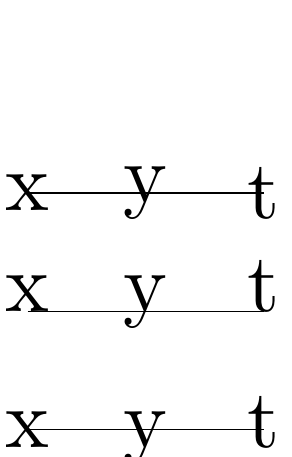
\begin{tikzpicture}[scale=3,transform shape]
	\path[use as bounding box, red] (0,0) rectangle (1, 1.7);
	% First, center alignment -> wobbles
	\draw[anchor=center] (0,1) node{x} -- (0.5,1) node{y} -- (1,1) node{t};
	
	% Second, base alignment -> no wobble, but too high
	\draw[anchor=base] (0,.5) node{x} -- (0.5,.5) node{y} -- (1,.5) node{t};
	
	% Third, mid alignment
	\draw[anchor=mid] (0,0) node{x} -- (0.5,0) node{y} -- (1,0) node{t};
\end{tikzpicture}
\end{document}